\documentclass[class=article,border=5pt,tikz]{standalone}
\usetikzlibrary{shapes}

\begin{document}

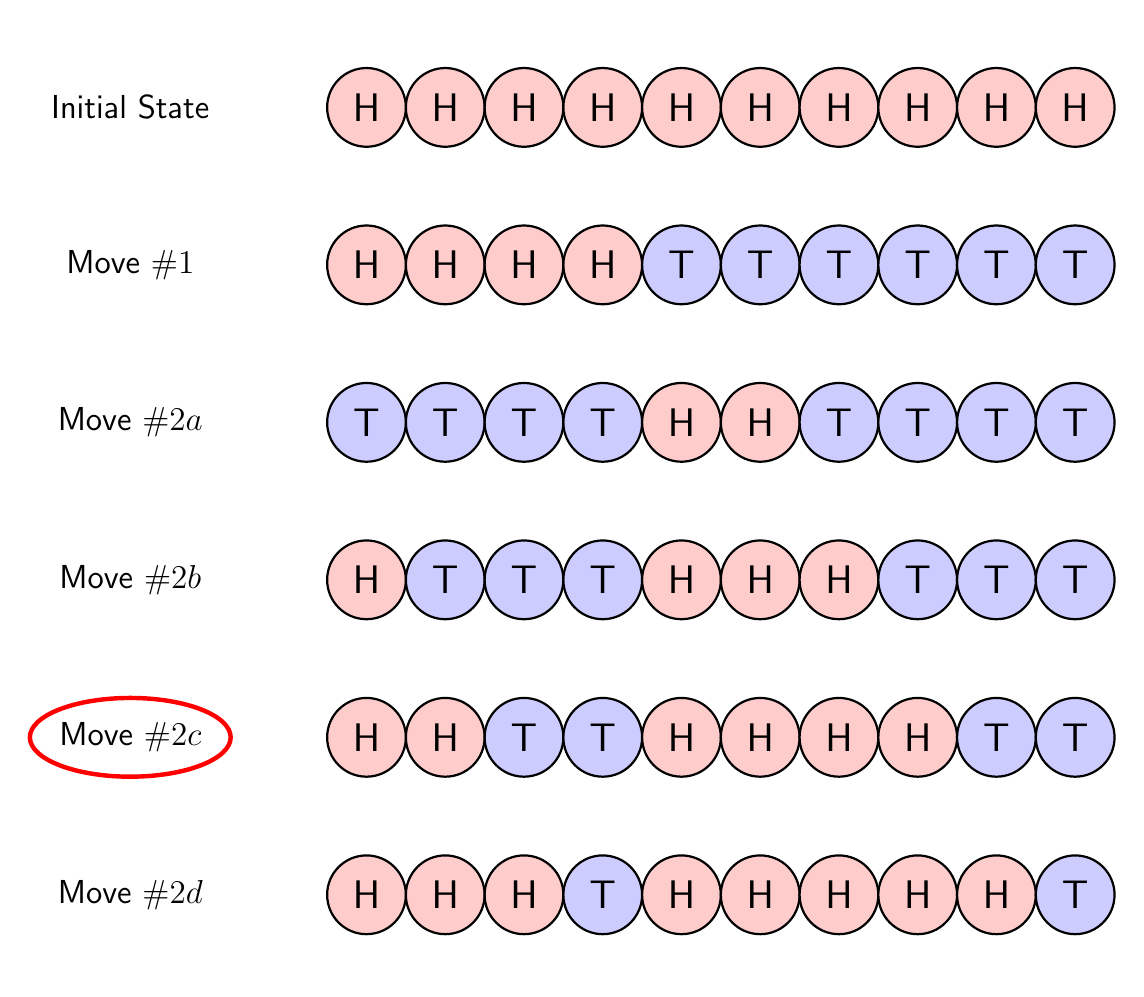
\begin{tikzpicture}[thick, scale=1,
    every node/.style = {circle, minimum size=10mm, inner sep=0mm, outer sep=0mm,
                         font=\sffamily\large, text=black},
          head/.style = {draw, fill=red!20, 
                         label=center:\textsf{\Large H}},
          tail/.style = {draw, fill=blue!20, 
                         label=center:\textsf{\Large T}},]%
  % 1st layout
  \node         at (-3,0) {Initial State};
  \node [head]  at (0,0) {};
  \node [head]  at (1,0) {};
  \node [head]  at (2,0) {};
  \node [head]  at (3,0) {};
  \node [head]  at (4,0) {};
  \node [head]  at (5,0) {};
  \node [head]  at (6,0) {};
  \node [head]  at (7,0) {};
  \node [head]  at (8,0) {};
  \node [head]  at (9,0) {};
  % 2nd layout
  \node         at (-3,-2) {Move $\# 1$};
  \node [head]  at (0,-2) {};
  \node [head]  at (1,-2) {};
  \node [head]  at (2,-2) {};
  \node [head]  at (3,-2) {};
  \node [tail]  at (4,-2) {};
  \node [tail]  at (5,-2) {};
  \node [tail]  at (6,-2) {};
  \node [tail]  at (7,-2) {};
  \node [tail]  at (8,-2) {};
  \node [tail]  at (9,-2) {};
  % 3rd layout
  \node         at (-3,-4) {Move $\# 2a$};
  \node [tail]  at (0,-4) {};
  \node [tail]  at (1,-4) {};
  \node [tail]  at (2,-4) {};
  \node [tail]  at (3,-4) {};
  \node [head]  at (4,-4) {};
  \node [head]  at (5,-4) {};
  \node [tail]  at (6,-4) {};
  \node [tail]  at (7,-4) {};
  \node [tail]  at (8,-4) {};
  \node [tail]  at (9,-4) {};
  % 4th layout
  \node         at (-3,-6) {Move $\# 2b$};
  \node [head]  at (0,-6) {};
  \node [tail]  at (1,-6) {};
  \node [tail]  at (2,-6) {};
  \node [tail]  at (3,-6) {};
  \node [head]  at (4,-6) {};
  \node [head]  at (5,-6) {};
  \node [head]  at (6,-6) {};
  \node [tail]  at (7,-6) {};
  \node [tail]  at (8,-6) {};
  \node [tail]  at (9,-6) {};
  % 5th layout
  \node [draw=red, ultra thick, ellipse]
                at (-3,-8) {Move $\# 2c$};
  \node [head]  at (0,-8) {};
  \node [head]  at (1,-8) {};
  \node [tail]  at (2,-8) {};
  \node [tail]  at (3,-8) {};
  \node [head]  at (4,-8) {};
  \node [head]  at (5,-8) {};
  \node [head]  at (6,-8) {};
  \node [head]  at (7,-8) {};
  \node [tail]  at (8,-8) {};
  \node [tail]  at (9,-8) {};
  % 4th layout
  \node         at (-3,-10) {Move $\# 2d$};
  \node [head]  at (0,-10) {};
  \node [head]  at (1,-10) {};
  \node [head]  at (2,-10) {};
  \node [tail]  at (3,-10) {};
  \node [head]  at (4,-10) {};
  \node [head]  at (5,-10) {};
  \node [head]  at (6,-10) {};
  \node [head]  at (7,-10) {};
  \node [head]  at (8,-10) {};
  \node [tail]  at (9,-10) {};
\end{tikzpicture}

\end{document}
